\header{
    \section{Caroline la putain} \label{caroline-la-putain}
    %
    
    \insertComment{Composée en 1770 par Marion de Mersan, adaptant des textes publiés en 1560 dans le Ciquiesme livre de chansons composé à troys parties.}{}
    
    %Ciquiesme livre de chansons composé à troys parties je laisse parce que ça à l'air fait exprès mais aucune idée
}

\enluminure{4}{\href{https://www.youtube.com/watch?v=9Pd1KcXYsF0}{A}}{h ! mes amis} qu'on verse à boire
\\Qu'on verse à boire et du bon vin
\\Tintin tintin tin ain' et tintin
\\Je m'en vais vous conter l'histoire
\\De Caroline la putain
\\Tintin tintain' et tintin
\\\\Son père était un machiniste
\\Au théâtre de l'Odéon
\\Tonton, tonton tontain' et tonton,
\\Sa mère était une fleuriste
\\Qui vendait sa fleur en bouton,
\\Tonton tontain' et tonton
\\\\Elle perdit son pucelage
\\Le jour de sa première communion
\\Tonton, tonton tontain' et tonton,
\\Avec un garçon de son âge,
\\Derrière les fortifications,
\\Tonton tontain' et tonton
\\\\A quatorze ans, suçant les pines,
\\Elle fit son éducation,
\\Tonton, tonton tontain' et tonton,
\\A dix-huit ans, dans la débine,
\\Elle s'engagea dans un boxon,
\\Tonton tontain' et tonton
\breakpage
A vingt-quatre ans, sur ma parole
\\C'était une fière putain
\\Tintin tintin tin tain' et tintin
\\Elle avait foutu la vérole
\\Aux trois-quarts du Quartier Latin
\\Tintin tintain' et tintin
\\\\Le marquis de la Couillemolle
\\Lui fit bâtir une maison
\\Tonton tonton tontain' et tonton
\\A l'enseigne du "Morpion qui vole"
\\Quelle chouette enseigne pour un boxon
\\Tonton tontain' et tonton
\\\\Elle voulut aller à Rome
\\Pour recevoir l'absolution
\\Tonton tonton tontain' et tonton
\\Le Pape était fort bien à Rome
\\Mais il était dans son boxon
\\Tonton tontain' et tonton
\\\\Et s'adressant au grand Vicaire
\\Elle dit : "j'ai trop prété mon con"
\\Tonton tonton tontain' et tonton
\\"Si tu l'as trop prété, ma chère,
\\Et bien ! Reprête-le moi donc !"
\\Tonton tontain' et tonton
\\\\Et la serrant entre ses cuisses,
\\Il lui donna l'absolution
\\Tonton tonton tontain' et tonton
\\Il attrapa la chaude pisse
\\Et trente six douzaines de morpions
\\Tonton tontain' et tonton
\breakpage
Elle finit cette tourmente
\\Entre les bras d'un marmiton
\\Tonton tonton tontain' et tonton
\\Elle mourut la pine au ventre
\\Le con fendu jusqu'au menton
\\Tonton tontain' et tonton
\\\\Et quand on la mit dans la bière
\\On vit pleurer tous ses morpions
\\Tonton tonton tontain' et tonton
\\Et quand on l'eût portée en terre
\\Ils s'arrachèrent les poils du con
\\Tonton tontain' et tonton
\\

\bigskip
\begin{figure}[h!]
\centering
   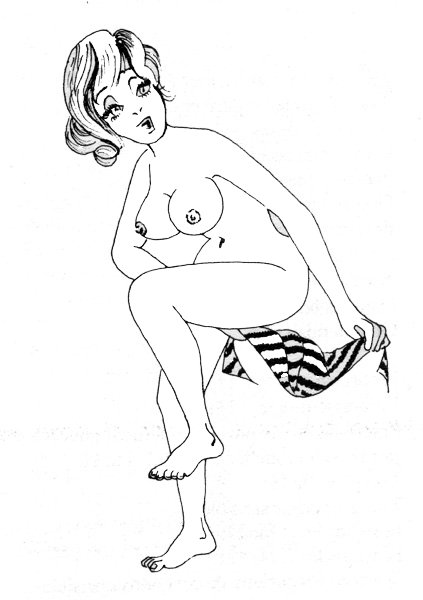
\includegraphics[width=0.7\textwidth]{images/image6.png}
 \end{figure}
 
\breakpage